%--------------------------------------------------------------------------------------------------
%
\chapter{Introduction}
%--------------------------------------------------------------------------------------------------

\emph{Pattern analysis} is the process of finding structure or regularity in a set of data. For example,
if each data instance represents a point in a vector space, we might be interested in the following question: does the dataset lie
in a lower dimensional subspace (does it admit a more compact representation)? In this case, the subspace represents a pattern (structure or regularity)
discovered in the data. Principal Component Analysis provides a solution to such a question.

This thesis deals with finding patterns in datasets that exhibit a \emph{multi-view} aspect: that is, for
each instance of data there are two or more representations (views) available. We refer to such datasets as
\emph{aligned} datasets. As an example of a two-view dataset, consider a dataset where each instance is represented by a visual image and
a textual description. Another example is a \emph{parallel multi-lingual corpus},
where given $n$ languages, each data instance consists of $n$ documents, one for each language and the documents are related by being
translations of each other. The patterns that we are interested in represent regularities within each representation
that are related across representations. For example, when dealing with text, a type of pattern that is often of interest
is a distribution over words from a fixed vocabulary, referred to as a \emph{topic vector}. Given a collection of documents
in a single language, a typical problem is to find relevant topic vectors that summarize the document collection. The multi-view
variant of the problem then corresponds to finding sets of multiple representations of topic vectors (one per language).
Methods that extract such multi-representation patterns represent the main subject of the thesis.

There are several possible applications of such an analysis. The patterns themselves can be of interest
for explorative analysis. For example, given an aligned dataset of fMRI brain scans and visual images that were
shown to the subjects as scans were taken, we can investigate how the brain functions by looking at
relationships between brain activation regions and patterns in visual images.
Another example of application is to use the multi-view patterns as maps into a
representation independent space. For example, representing visual images and textual descriptions in the same
space can be used for cross-modal information retrieval, where we map queries and document/image collections
to the same space where standard similarity measures (such as cosine similarity) can be used for information
retrieval. In addition, the optimization problem related to a particular generalization of CCA which we study
appears in applications that range from control theory, blind source separation, multiple subject fMRI analysis.

\section{Overview and Questions Addressed}

We will now provide a high-level overview of the results presented in the thesis and highlight the related work
that motivated or enabled the results, all of which is summarized in Figure~\ref{fig:position_of_work}.
Canonical Correlation Analysis (CCA)~\cite{Hotelling}, a well established method that looks for patterns in two-view
datsets, has been extended by other authors in several ways: a nonlinear extension was proposed in~\cite{FBMJ}, which
was later applied to text in~\cite{vinokourov2002inferring}. It has been extended to more than two sets of variables
in~\cite{Horst}, where a formulation called \emph{Sum of Correlations} (SUMCOR) was presented, together with an iterative
algorithm to finding local solutions, known as the \emph{Horst algorithm}. Results on global optimality of a subset
of SUMCOR problems was established in~\cite{GlobalMEP} and~\cite{GlobalMEP2}. Several alternative generalizations
of CCA were proposed in~\cite{Kettenring}, where the most relevant extension to the thesis is the
\emph{Sum of Squared Correlations} (SSCOR).

The thesis starts with two questions:
\begin{itemize}
\item How can we extend the Horst algorithm to handle nonlinear patterns and how to find several sets of canonical vectors? Does the extension provably converge?
\item What is the computational complexity of the SUMCOR problem formulation?
\end{itemize}
We present an extension that is closely related to~\cite{FBMJ} and show that it does converge to local solutions. We prove that in
general the computational complexity of the SUMCOR problem is NP-hard.
 In light of these results, several questions arose:
\begin{itemize}
\item Can we find a convex relaxation of the problem?
\item Can we obtain computationally tractable bounds on the SUMCOR objective?
\end{itemize}
We show how to relax the problem to an instance of a Semidefinite Programming (SDP), whose solutions yield
computable bounds on global optimality. The results related to SUMCOR complexity and SDP relaxations
are available in~\cite{DBLP:journals/corr/abs-1302-0974} and submitted for publication.

Applying the theory to practice opened up the following questions:
\begin{itemize}
\item How to apply the SDP bounds to high dimensional data?
\item How can one use the methods to perform cross-lingual document analysis?
\item How does one handle missing data?
\end{itemize}
To address the first question, we proposed a random projection based preprocessing step that reduces the number
of variables in the SDP derived from a SUMCOR problem instance that makes the computations scalable. Addressing
the second question, we present the methodology for building cross-lingual similarity functions and apply it
to the task of cross-lingual cluster linking. The application is relevant to global analysis of high-volume
multi-lingual news streams.

We address the problem of missing data in our application to cross-lingual text mining for datasets where
data was missing in a structured way and show that under certain assumptions, the SSCOR problem formulation
can be reduced to a low-dimensional eigenvalue problem. The results related to SSCOR reduction and
cross-lingual applications are available in~\cite{rupnikJAIR}.
An alternative application of the SSCOR reformulation to cluster linking is published in~\cite{Belyaeva201564}.

\begin{figure}[t]
\centering
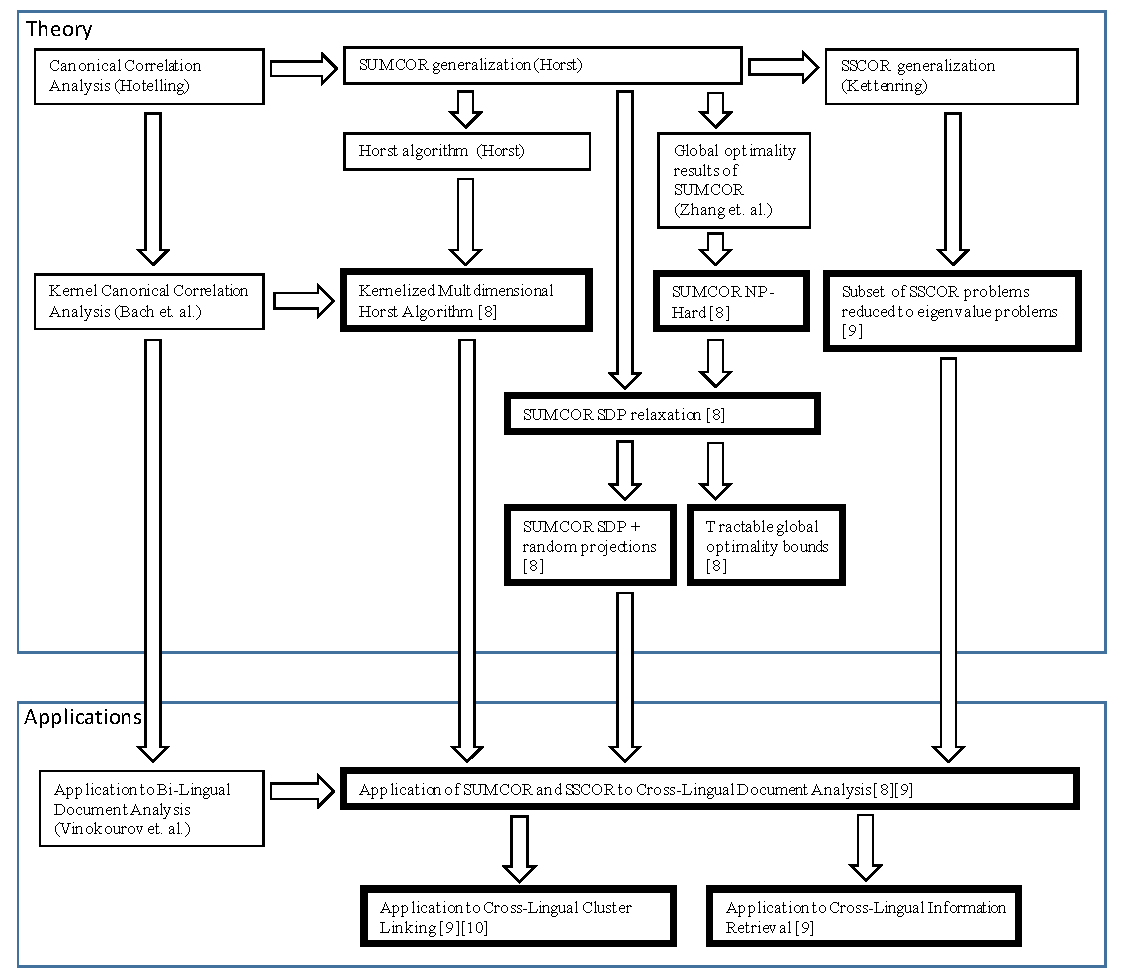
\includegraphics[width=1\textwidth]{figures/position_of_work.pdf}
\caption[The main contributions and related work]{The main contributions, represented by text boxes with thick border, are
positioned with respect to the related work.}
\label{fig:position_of_work}
\end{figure}

\section{Scientific Contributions}

We now list the main scientific contributions of the thesis:
\begin{itemize}
\item A novel algorithm based on the Horst algorithm that can extract several sets of nonlinear patterns
\item A proof that in general the Sum of Correlations problem is NP-hard
\item A semidefinite programming relaxation of the SUMCOR problem and
several new bounds on global optimization of the SUMCOR problems
\item A novel approach to apply the SDP bounds on high-dimensional data
\item A novel approach to building cross-lingual similarity functions and its application to cross-lingual information retrieval and cross-lingual cluster linking
\item Addressing the missing data problem, a novel reduction of a subset of SSCOR problems to eigenvalue problems
\end{itemize}

\section{Thesis Structure}

The rest of the thesis is structured as follows. Chapter~\ref{chap:notation} introduces notation and some
definitions. For background we describe three pattern analysis methods that are the most relevant
for the thesis and explain how they can be adapted for analysis of nonlinear patterns in Chapter~\ref{chap:background}. Chapter~\ref{chap:extensions}
introduces a central problem of the thesis: generalizations of Canonical Correlation Analysis (CCA) and the original
contributions that extend the method to nonlinear and higher-dimensional setting. In Chapter~\ref{chap:relaxations}
we prove the result on the complexity of a particular generalizations and study global optimality guarantees based
on semidefinite relaxations. Chapter~\ref{chap:crosslingual} discusses an application of multiview learning
to building cross-lingual similarity models. We show how a particular structure of the data can be exploited
to express a particular generalization of CCA as an eigenvector problem. Chapter~\ref{chap:applications} then
shows how the cross-lingual similarity measures can be used to perform cross-lingual cluster linking, relevant
for large scale monitoring of global news in multiple languages. In Chapter~\ref{chap:experiments} several experiments
are presented both on synthetic and real datasets. Finally, Chapter~\ref{chap:conclusions} concludes the thesis
and discusses possible future directions. 